The baseline design of \nuprismlite is an outer detector (OD) volume with radius of 5 m and 
height of 14 m, and an inner detector (ID) volume with a radius of 3 m and height of 10 m, located
1 km from the T2K target.  We have carried out a simulation of events in the 
\nuprismlite ID and OD volumes, as well as the surrounding earth to study the event pile-up
in \nuprismlite.  The simulation is carried out for the earth+\nuprismlite 
geometry shown in Fig.~\ref{fig:sand_geom}.  The flux at the upstream end of the volume is simulated
using the JNUBEAM package with horn currents set to 320 kA.  Interactions in the earth and detector 
volumes are generated using the same tools from the NEUT package used for ND280 neutrino vector
generation.  The earth volume is filled with SiO$_{2}$ with a density of 1.5 g/cm$^{3}$.  The water volume
has three detector sub-volumes: the ID detector, the OD detector and an intermediate volume.
The vertical position of the detector volumes in the water column can be adjusted to study the
event pile-up at different off-axis angles.  A GEANT4 simulation of the particles from the neutrino
vectors is carried out and all particles with visible energy greater than 10 MeV are recorded if they 
originate in any of the detector volumes or cross any of the detector volume boundaries.

\begin {figure}[htbp]
  \begin{center}
    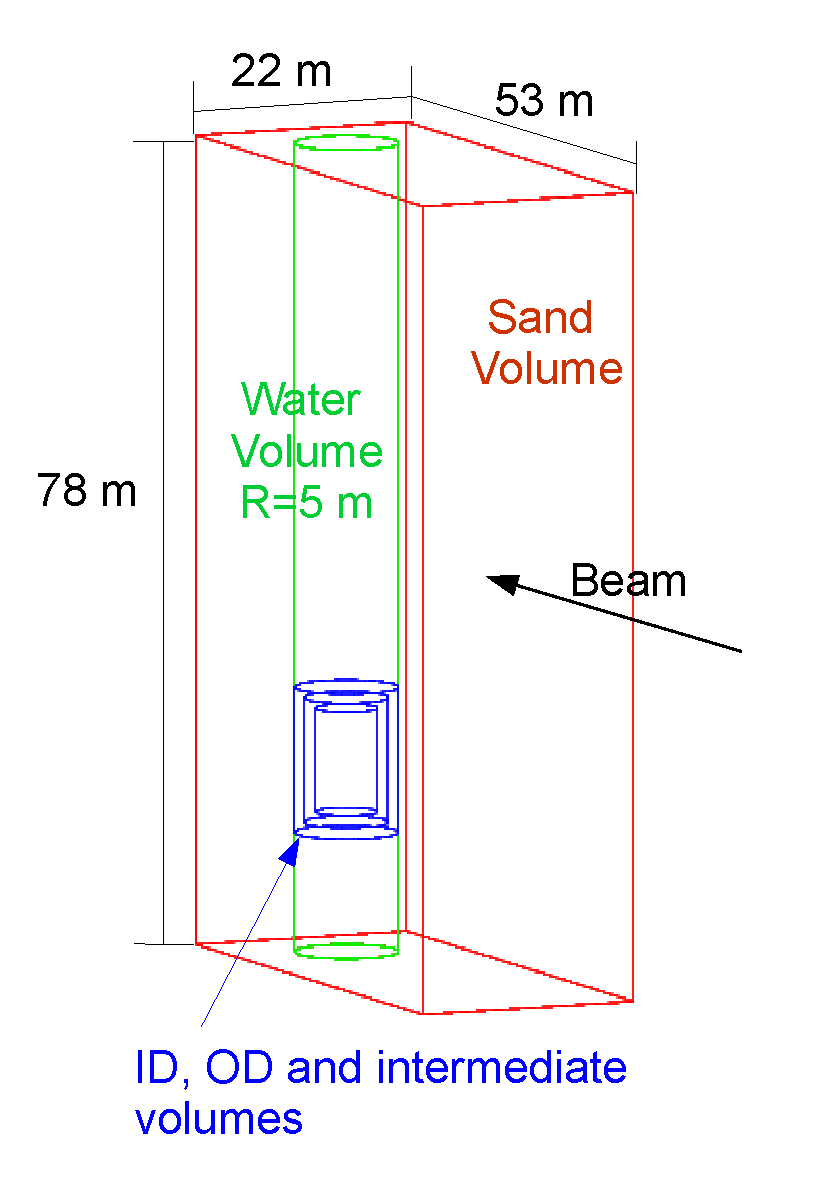
\includegraphics[width=9cm]{figures/nuprism_sand_geom.pdf}
    \caption{The GEANT4 geometry used in the pile-up simulation.}
    \label{fig:sand_geom}
  \end{center}
\end {figure}


We break up the visible events into five categories for the pile-up studies:
\begin{enumerate}
\item Events originating outside of the ID and entering the ID.
\item Events originating inside the ID with visible particles escaping the ID.  These are called partially contained (PC) ID events.
\item Events originating inside the ID with no visible particles escaping the ID.  These are called fully contained (FC) ID events.
\item Events originating in the OD with no visible particles entering the ID.  
\item Events originating outside the OD with visible particles entering the OD, but not the ID.
\end{enumerate}
The first three categories represent the event rate in the ID, while all but the second category represent the event rate
in the OD.  Table~\ref{tab:pileup} shows the simulated event rates per $2.5\times10^{13}$ protons on target, the assumed protons per bunch for full
750 kW operation.  Rates are shown for the \nuprismlite configurations where the ID covers off-axis angle ranges of 0.0-0.6, 1.0-1.6,
2.0-2.6 or 3.0-3.6 degrees.  While the current design does not include a pit that extends to on-axis, the 0.0-0.6 degree position is used
to make comparisons to the INGRID event rates.

\begin{table*}
\begin{center}
\caption{The event rates per 2e13 POT for \nuprismlite with horn currents at 320 kA.}
\label{tab:pileup}
\begin{tabular}{l|c|c|c|c|c}
\hline
Off-axis Angle ($^{\circ}$) & Entering ID & PC ID  & FC ID  & OD Contained  & Entering OD    \\ \hline
0.0-0.6                     & 0.4179      & 0.2446 & 0.3075 & 1.2904        & 0.7076 \\
1.0-1.6                     & 0.1005      & 0.0550 & 0.0741 & 0.3410        & 0.1939 \\
2.0-2.6                     & 0.0350      & 0.0198 & 0.0230 & 0.1234        & 0.0635 \\
3.0-3.6                     & 0.0146      & 0.0092 & 0.0156 & 0.0564        & 0.0291 \\ \hline
\end{tabular}
\end{center}
\end{table*}

For the off-axis angle 1.0-1.6 degree position, the total rate of ID+OD visible events in a spill (8 bunches) is 6.12.  If a bunch contains 
an event, the probability that the next bunch contains at least one visible event is 53\%.  This suggests that \nuprismlite should employ
deadtime-less electronics that can record events in neighboring bunches and that the after-pulsing of PMTs
should be carefully considered. 
The rate of ID events per bunch is 0.230 and the probability of two or more visible ID
events in a single bunch with at least one visible event is 20\%.  Hence, most bunches will not require the reconstruction of multiple interactions
in the ID volume.  
However, the probability of 2 or more ID events per spill is 84\%, so the reconstruction of out of time events such
as decay electrons needs to be carefully studied.  Decay electrons in a spill may potentially be matched to their parent
 interactions using both spatial and timing information.  For interactions inside the ID, a spatial likelihood matching
 the decay electron to the primary vertex may be constructed based on the reconstructed decay electron vertex position and 
the reconstructed primary vertex or reconstructed stopping point of the candidate muons or charged pions in the event. For decay electrons
 originating from muons produced outside of the ID, a similar spatial likelihood may be constructed using OD light, ID light, and hits from 
scintillator panels (if they are installed between the OD and ID) from the entering particle.   Since the muon mean lifetime (2.2 $\mu$s) is 
shorter than the spill length (~5 $\mu$s), there will also be statistical power to match decay electrons to their primary vertex based on 
the time separation of the decay electron vertex and primary vertex.  On the other hand, the muon lifetime may provide a cross-check for the 
spatial matching of primary and decay electron vertices since significant mismatching would tend to smear the time separation distribution 
beyond the muon lifetime.  Studying the matching of decay electrons to primary interactions is a high priority and work is underway to address 
this issue with a full simulation of \nuprism and the surrounding rock.


The rate of events producing light in the OD is 0.690 per bunch.  Hence, the 
probability that an FC ID event will have OD activity in the same bunch is 50\%.  Neglecting out of time events,
the rejection rate of FC ID events would be 50\% if a veto on any OD activity in the bunch is applied.  This rejection rate falls
to 21\% and 10\% in the 2.0-2.6 and 3.0-3.6 degree off-axis positions respectively.  Of the OD events, about 30\% are entering
from the surrounding earth, and most of those are muons.  The scintillator panels may be used to relax the veto on these types of 
pile-up events by providing additional spatial and timing separation between the OD and ID activity in the same bunch.
If the veto can be removed for all events entering the OD from the earth,
then rejection rates due to OD pile-up drop to 39\%, 16\% and 8\% for the 1.0-1.6, 2.0-2.6 and 3.0-3.6 degree
off-axis angle positions respectively.

We can cross-check the estimated \nuprism event rates by extrapolating from the event rates observed by INGRID.  We assume that
the rate of interactions inside the detector will scale with the detector mass, and the rate of entering events from the earth
will scale with the cross-sectional area of the detector.  The rates should also scale with $1/d^{2}$, were $d$ is the
distance from the average neutrino production point to the detector, about 240~m for INGRID and 960~m for \nuprism. 
INGRID observes 1.74 neutrino events per $1\times10^{14}$ POT in 14 INGRID modules with a total mass of $5.7\times10^4$ kg.  For an OD mass
of $8.2\times10^5$~kg, we extrapolate the INGRID rate, assuming 60\% detection efficiency in INGRID, to obtain 0.66 interactions 
in the OD for each $2.5\times10^{13}$ POT bunch.  The simulated rate of visible OD interactions in \nuprismlite is 1.50 and 0.39 for
the 0.0-0.6 and 1.0-1.6 degree positions respectively.  Since INGRID covers an angular range of about $\pm1$ degree, it is
reasonable that the extrapolated value from INGRID falls between the simulated \nuprismlite values at these two positions.

INGRID also observes a event rate from earth interactions of 4.53 events per $1\times10^{14}$ POT in 14 modules with a cross-sectional area
of 21.5~m$^{2}$.  These earth interaction candidates are INGRID events failing the upstream veto and fiducial volume cuts.  The selection
of entering earth-interaction events is $>99$\% efficient and 85.6\% pure.  Scaling to the OD cross-sectional area and
distance while
correcting for the efficiency and purity gives a rate of 0.31 events entering the OD per bunch.  The rate from
the \nuprism pile-up simulation is 0.903 or 0.239 for the 0.0-0.6 and 1.0-1.6 degree positions respectively.  Once again, the extrapolated
INGRID rate falls between the simulated rates for these two \nuprismlite positions.

In summary, the event pile-up rates for \nuprism appear manageable.  Even for the most on-axis position and high power beam, most bunches
with interactions will only have a single interaction with visible light in the ID.  The OD veto rate from pile-up can be as large as 50\%,
hence careful studies of the OD veto are needed.
The OD veto rate may be reduced and better understood with the inclusion of scintillator panels at the outer edge of the OD or at the OD/ID 
boundary.  The electronics for \nuprismlite should be deadtime-less to handle multiple events per spill.  

Further studies of the event rates will be carried out.  These will include the study of entering neutral particles to be used
in the optimization of the OD and fiducial volume sizes, more realistic studies of how the scintillator panels may be used to
optimize the OD veto cut, and updates to the earth density to better reflect the surveyed density of the rock strata at potential \nuprism sites.  

 
